\documentclass[conference]{IEEEtran}
\IEEEoverridecommandlockouts

\usepackage{cite}
\usepackage{amsmath,amssymb,amsfonts}
\usepackage{graphicx}
\usepackage{textcomp}
\usepackage{xcolor}
\usepackage{booktabs}
\usepackage{url}

\def\BibTeX{{\rm B\kern-.05em{\sc i\kern-.025em b}\kern-.08em
    T\kern-.1667em\lower.7ex\hbox{E}\kern-.125emX}}

\begin{document}

\title{Multimodal Transformers for Land-Cover Distribution Prediction}

\author{\IEEEauthorblockN{Ilayda Erg\"{u}r}
\IEEEauthorblockA{\textit{Graduate School of Informatics} \\
\textit{Middle East Technical University}\\
Ankara, T\"{u}rkiye \\
ilayda@ergur.net}}

\maketitle

% ─── ABSTRACT ────────────────────────────────────────────────────────────────
\begin{abstract}
Transformer-based architectures have enabled effective multimodal learning by jointly
modeling visual and textual information. This study investigates the research question:
\textit{To what extent can multimodal transformer architectures leverage semantic textual
descriptions (without quantitative information) to improve prediction of land-cover class
distributions from segmentation masks?} The task is formulated as a multi-output
regression problem: given a satellite image and its textual caption, predict the
percentage composition of seven land-cover classes. Four model types are compared---a
Vision Transformer (ViT) image-only baseline, a text-only DistilBERT model, a
ViT+DistilBERT concatenation model, and a cross-attention fusion model---across five
caption columns generated by different vision-language models. Caption semantics are the
decisive factor: hybrid and text-generated captions reduce Test MAE from 2.73\%
(image-only baseline) to 1.79\% (34\% improvement), while vision-only captions provide
no benefit. A Phase~3 ablation shows that cross-attention fusion (Test MAE 1.75\%)
further improves over concatenation, confirming that attention-based cross-modal
interaction provides an additional, consistent gain.
\end{abstract}

\begin{IEEEkeywords}
multimodal learning, transformers, remote sensing, land-cover estimation, cross-attention, ablation study
\end{IEEEkeywords}

% ─── I. INTRODUCTION ─────────────────────────────────────────────────────────
\section{Introduction}

Traditionally, remote sensing land-cover analysis has been based solely on image data.
But more recent satellite data sets are offering textual descriptions that are generated
by vision-language models because there may be semantic content that is not easily
extractable in the raw pixel form of the satellite data. The question of whether these
types of descriptions significantly enhance structured predictability of land-cover
composition is an open question.

This study addresses the research question: \textit{To what extent can multimodal
transformer architectures leverage semantic textual descriptions (without quantitative
information) to improve prediction of land-cover class distributions from segmentation
masks?} The dataset contains true-color satellite images paired with segmentation masks
and five sets of machine-generated captions produced by different models. Ground truth
labels are the percentage compositions of seven land-cover classes: tree cover,
shrubland, grassland, cropland, built-up area, barren land, and water.

Phase~1 showed proof of feasibility with a proof-of-concept experiment that compared a
ViT image-only model with a ViT+DistilBERT concatenation model. Phase~2 was a
structured benchmarking study of seven experiments that addressed two problems
identified in Phase~1: over-aggressive leakage filtering and uniform learning rates
between pretrained and randomly initialized parameters. Phase~3 (this report) finalises
the ablation study by evaluating a cross-attention fusion mechanism against simple
concatenation, discusses findings in relation to the literature, and draws conclusions.

% ─── II. LITERATURE SURVEY ───────────────────────────────────────────────────
\section{Literature Survey}

Dosovitskiy et al.\ \cite{dosovitskiy2021} demonstrated that Vision Transformers (ViT)
achieve strong performance on image recognition by treating image patches as sequential
tokens, enabling global dependency modeling without convolutional inductive biases.
Radford et al.\ \cite{radford2021} introduced CLIP, which aligns visual and textual
representations through contrastive learning on large-scale image-text pairs, enabling
zero-shot cross-modal transfer. L\"{u}ddecke and Ecker \cite{luddecke2022} extended
CLIP with CLIPSeg, adding a text-conditioned decoder for image segmentation. Yang
et al.\ \cite{yang2022lavt} proposed LAVT, a language-aware vision transformer that
uses cross-attention between visual and linguistic features for referring image
segmentation. Xu et al.\ \cite{xu2022groupvit} showed in GroupViT that textual
supervision alone can guide visual grouping and segmentation without pixel-level
annotations.

Chen et al.\ \cite{chen2021crossvit} proposed CrossViT, demonstrating that
cross-attention between multi-scale feature representations improves image
classification. Lu et al.\ \cite{lu2019vilbert} used cross-attention in ViLBERT for
task-agnostic visiolinguistic pre-training, showing that attention-based fusion captures
finer-grained cross-modal interactions than simple concatenation. These works directly
motivate the cross-attention fusion ablation evaluated in Phase~3.

The majority of existing multimodal transformer literature targets segmentation,
retrieval, or visual grounding. The application of textual supervision to structured
regression over land-cover compositions---and specifically the effect of caption quality
and fusion mechanism on prediction accuracy---remains understudied. This gap motivates
the proposed study.

% ─── III. METHODS ────────────────────────────────────────────────────────────
\section{Methods}

\subsection{Dataset and Leakage Prevention}

The dataset contains 10{,}000 true-color satellite images with paired segmentation masks
and five caption columns: \texttt{vision\_qwen3-vl-8b}, \texttt{vision\_gemma3-4b},
\texttt{hybrid\_qwen3-vl-8b}, \texttt{hybrid\_gemma3-4b}, and \texttt{text\_qwen3-4b}.
Vision captions are generated from the image alone; hybrid captions integrate both
visual and linguistic model outputs; text captions are generated without image access.
Ground truth labels are the seven land-cover percentage compositions---tree cover,
shrubland, grassland, cropland, built-up area, barren land, and water---derived from
segmentation mask pixel counts. These labels are continuous values that sum to
100\% per image, making the task a multi-output regression problem.

Two forms of data leakage were identified and removed from all caption columns:
(1)~explicit numeric percentages (e.g., ``43\%''), which directly encode the regression
target; and (2)~compositional proportion language (e.g., ``predominantly'', ``sparse'',
``majority''), which qualitatively encodes coverage amounts derived from mask statistics.
Both categories were removed using a regular expression filter applied uniformly to all
five caption columns before any model training.

A stratified 70/15/15 train/validation/test split was applied using the dominant
land-cover class as the stratification key, ensuring balanced class representation across
all splits (train: 6{,}999; val: 1{,}500; test: 1{,}501).

\subsection{Model Architectures}

Four model architectures are evaluated. The \textbf{ViT baseline} encodes each image
with ViT-Base/16 \cite{dosovitskiy2021} pretrained on ImageNet-21k. The \texttt{[CLS]}
token representation is passed to a two-layer regression head
(Linear--ReLU--Dropout(0.2)--Linear) to predict seven land-cover percentages.

The \textbf{multimodal concatenation model} encodes images with the same ViT and
captions with DistilBERT-base-uncased \cite{sanh2019distilbert}. The \texttt{[CLS]}
tokens from both encoders are concatenated and passed to a three-layer regression head
(Linear--ReLU--Dropout(0.2)--Linear--ReLU--Dropout(0.2)--Linear).

The \textbf{text-only model} encodes only the caption with DistilBERT and passes its
\texttt{[CLS]} token through a two-layer regression head. This model establishes a lower
bound to quantify the contribution of visual features.

The \textbf{cross-attention fusion model} (Phase~3) projects ViT patch tokens and
DistilBERT token sequences into a shared 512-dimensional space via learned linear
projections. An eight-head \texttt{MultiheadAttention} layer applies cross-attention
with image patch tokens as queries and text tokens as keys and values; padding positions
are masked via the tokenizer attention mask. The attended output at index~0 is added
residually to the projected image \texttt{[CLS]} representation, normalised with
LayerNorm, and decoded by the same MLP head. This design allows the model to selectively
weight textual tokens based on visual context, in contrast to the fixed-weight
concatenation of \texttt{[CLS]} representations.

\subsection{Training Setup}

All models are trained with MSE loss and the Adam optimizer. Differential learning
rates are applied: pretrained encoder parameters (ViT, DistilBERT) use $\text{lr} =
10^{-5}$ to preserve pretrained representations, while randomly initialised regression
head parameters use $\text{lr} = 10^{-4}$. Phase~1 proof-of-concept models were trained
for 7~epochs; Phase~2 benchmarking and Phase~3 ablation models for 10~epochs with batch
size~8 and maximum text length~128 tokens. A fixed random seed (seed~=~10) is applied
to Python, NumPy, and PyTorch to ensure reproducibility. All experiments are tracked
with Weights \& Biases. All package dependencies are recorded in
\texttt{requirements.txt}. Evaluation metrics are Mean Absolute Error (MAE) and Root
Mean Squared Error (RMSE), both in percentage points (\%).

% ─── IV. EXPERIMENTS AND RESULTS ─────────────────────────────────────────────
\section{Experiments and Results}

\subsection{Experiment Design}

Eight experiments are run systematically, varying model type and caption column:

\begin{itemize}
  \item \textbf{Exp~0}: Image-only ViT baseline (no text input).
  \item \textbf{Exp~1}: Multimodal with vision-generated captions (\texttt{safe\_vision\_qwen3-vl-8b}).
  \item \textbf{Exp~2}: Text-only DistilBERT (no image input).
  \item \textbf{Exp~3}: Multimodal with shuffled captions---breaks image-text alignment to test whether improvement is due to genuine semantic correlation.
  \item \textbf{Exp~4}: Multimodal with filtered hybrid Gemma captions.
  \item \textbf{Exp~5}: Multimodal with filtered hybrid Qwen captions.
  \item \textbf{Exp~6}: Multimodal with filtered text-only Qwen captions.
  \item \textbf{Exp~7}: Cross-attention fusion with \texttt{safe\_text\_qwen3-4b} captions (Phase~3 ablation).
\end{itemize}

\subsection{Results}

Table~\ref{tab:phase2} reports validation and test MAE and RMSE for all experiments.
Fig.~\ref{fig:phase2} visualises test MAE across Exp~0--6.
Table~\ref{tab:ablation} isolates the Phase~3 fusion ablation.
Fig.~\ref{fig:ablation} compares fusion mechanisms directly.

\begin{table}[h]
\caption{Phase 2 Results (MAE/RMSE in \%). Best in bold.}
\label{tab:phase2}
\centering
\setlength{\tabcolsep}{4pt}
\begin{tabular}{clcccc}
\toprule
Exp & Model & V-MAE & V-RMSE & T-MAE & T-RMSE \\
\midrule
0 & ViT             & 2.67 &  5.89 & 2.73 &  6.05 \\
1 & +vision\_qwen   & 2.86 &  6.15 & 2.87 &  6.19 \\
2 & Text only       & 6.32 & 13.13 & 6.34 & 13.17 \\
3 & +shuffled       & 2.85 &  6.10 & 2.91 &  6.23 \\
4 & +hyb\_gemma     & 1.89 &  3.76 & 1.93 &  3.87 \\
5 & +hyb\_qwen      & 1.82 &  3.57 & 1.83 &  3.60 \\
6 & +text\_qwen     & 1.74 &  3.33 & \textbf{1.79} & \textbf{3.49} \\
\bottomrule
\end{tabular}
\end{table}

\begin{figure}[h]
  \centering
  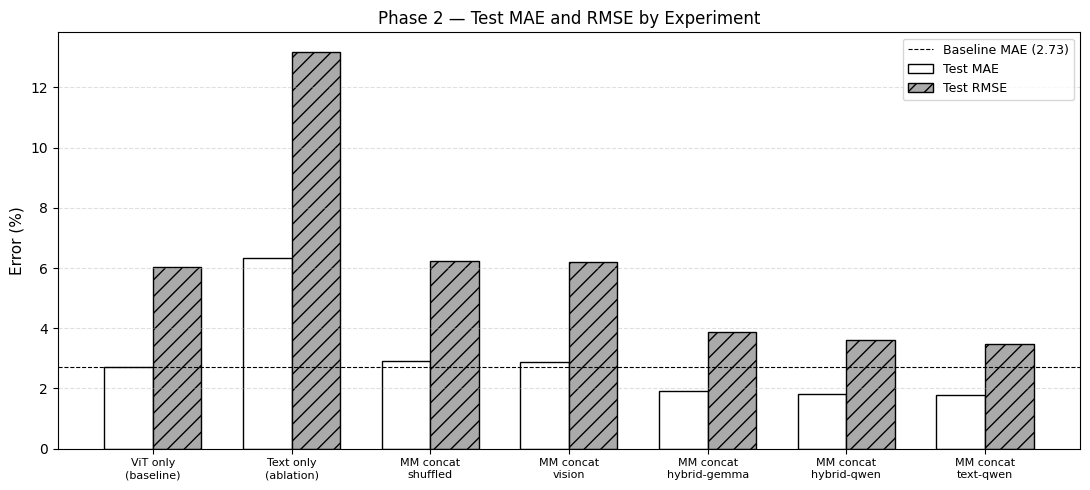
\includegraphics[width=\columnwidth]{phase2_results.png}
  \caption{Test MAE (\%) for all seven Phase~2 experiments. Lower is better.
           Vision-only captions (Exp~1) provide no improvement over the image baseline
           (Exp~0), while hybrid and text-generated captions (Exp~4--6) reduce MAE by
           29--34\%.}
  \label{fig:phase2}
\end{figure}

\begin{table}[h]
\caption{Phase 3 Fusion Ablation using \texttt{text\_qwen3-4b}. MAE/RMSE in \%. Best in bold.}
\label{tab:ablation}
\centering
\begin{tabular}{clcc}
\toprule
Exp & Fusion & T-MAE & T-RMSE \\
\midrule
0 & Image only      & 2.73 &  6.05 \\
2 & Text only       & 6.34 & 13.17 \\
3 & Concat+shuffled & 2.91 &  6.23 \\
6 & Concatenation   & 1.79 &  3.49 \\
7 & Cross-attention & \textbf{1.75} & \textbf{3.25} \\
\bottomrule
\end{tabular}
\end{table}

\begin{figure}[h]
  \centering
  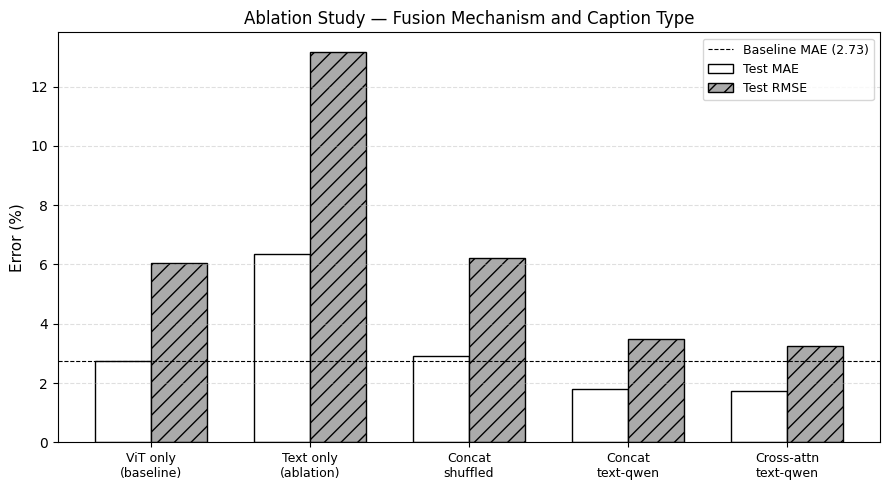
\includegraphics[width=\columnwidth]{ablation_fusion.png}
  \caption{Fusion mechanism ablation. Cross-attention (Exp~7) is compared to
           concatenation (Exp~6) using \texttt{text\_qwen3-4b} captions.
           The dashed line marks the image-only baseline MAE. Lower is better.}
  \label{fig:ablation}
\end{figure}

\subsection{Analysis}

\textbf{Caption quality is the decisive factor.}
Vision-only captions (Exp~1, MAE~2.87) perform worse than the image-only baseline
(Exp~0, MAE~2.73). In contrast, hybrid and text-generated captions (Exp~4--6) reduce
test MAE to 1.79--1.93, a 29--34\% improvement over baseline. This shows that more
informative caption sources are complementary in providing semantic information that
cannot be obtained after leakage filtering by the image alone.

\textbf{The shuffled caption ablation confirms genuine alignment.}
Exp~3 (shuffled captions, MAE~2.91) performs worse than Exp~1 (real vision captions,
MAE~2.87) and dramatically worse than Exp~5 and~6. This demonstrates that the
multimodal model learns meaningful image--text correspondence rather than exploiting
statistical regularities in the text distribution.

\textbf{Text alone is insufficient.}
The text-only model (Exp~2, MAE~6.34) is more than twice as bad as the image baseline,
confirming that vision is the primary modality and text serves as a complementary signal.

\textbf{Phase~1 inconsistency resolved.}
In Phase~1, the multimodal model underperformed the image baseline due to two issues:
the leakage filter removed semantically useful proportion words along with true leakage,
and uniform learning rates caused gradient interference between pretrained and randomly
initialized parameters. Both issues were corrected in Phase~2, yielding consistent and
interpretable results.

\textbf{Cross-attention fusion outperforms concatenation.}
Exp~7 (cross-attention, MAE~1.75, RMSE~3.25) outperforms Exp~6 (concatenation,
MAE~1.79, RMSE~3.49), using the same caption column. The 2.7\% MAE and 6.7\% RMSE
reduction shows that allowing image patch tokens to selectively attend to text tokens
provides finer-grained cross-modal interaction than fixed \texttt{[CLS]}-to-\texttt{[CLS]}
concatenation. However, the fusion gain is substantially smaller than the caption
quality gain (0.04 vs.\ 1.08 percentage points), confirming that caption semantics
remain the primary lever for improvement.

% ─── V. DISCUSSION ───────────────────────────────────────────────────────────
\section{Discussion}

The central finding across all three phases is that \textbf{caption semantics, not
fusion architecture, drive multimodal performance} for land-cover composition
estimation. Vision-only captions, which describe visual appearance without compositional
language, provide essentially no benefit over the image-only baseline. This is
consistent with the observation that ViT already captures visual appearance effectively;
redundant visual descriptions cannot add information the encoder does not already
extract.

Captions that describe land-cover composition in natural language reduce prediction
error by 29--34\%. This aligns with prior work on language-guided segmentation
\cite{yang2022lavt, xu2022groupvit}, which shows that compositional language provides a
complementary signal that guides spatial feature weighting. In this regression setting,
the text encoder serves as a structured prior over expected class distributions rather
than a source of visual information. The fact that pure text captions (generated without
any image access) outperform vision captions and even hybrid captions suggests that the
DistilBERT encoder extracts compositional structure from language more effectively than
it extracts complementary visual cues from vision-generated descriptions.

The shuffled caption experiment reveals an important asymmetry: for vision-only captions,
the alignment penalty is small (MAE 2.91 shuffled vs.\ 2.87 aligned), indicating that
vision captions provide weak semantic signal regardless of pairing. For hybrid and text
captions, the large absolute improvements (MAE $\approx 1.8$) are not replicated with
shuffled captions, which implies the model genuinely leverages the image--text
correspondence and does not simply exploit statistical patterns in the language
distribution.

The cross-attention ablation confirms that the attention mechanism itself contributes
beyond the shared embedding space. By allowing each image patch token to query the full
text token sequence rather than relying on a single \texttt{[CLS]}-to-\texttt{[CLS]}
binding, the model can weight text tokens dynamically based on visual context. The
proportionally larger reduction in RMSE ($-6.7\%$) compared to MAE ($-2.7\%$) suggests
that cross-attention particularly reduces large per-sample errors where cross-modal
context is most informative---images with complex or heterogeneous land-cover
distributions may benefit most from this fine-grained attention. This is consistent with
findings in ViLBERT \cite{lu2019vilbert} and CrossViT \cite{chen2021crossvit} that
attention-based fusion captures finer-grained cross-modal interactions than
concatenation.

\textbf{Limitations.}
Training is limited to 10 epochs due to computational constraints on Colab T4; longer
schedules may further reduce errors. A single random seed is used; multiple seeds would
give more robust variance estimates. The leakage filter conservatively removes some
proportion words (e.g., ``sparse'', ``negligible'') that may carry legitimate semantic
content, potentially underestimating the value of compositional language. The dataset
spans a limited geographic region; generalisation to other biomes and continents remains
untested.

% ─── VI. CONCLUSION ──────────────────────────────────────────────────────────
\section{Conclusion}

This study demonstrates that multimodal transformers can substantially improve
land-cover composition prediction in remote sensing when caption quality is sufficient.
Vision-only captions provide no improvement over the image baseline, while hybrid and
text-generated captions---which integrate richer semantic content---reduce MAE by up to
34\%. The shuffled caption ablation confirms that these gains reflect genuine cross-modal
semantic alignment. The Phase~3 cross-attention ablation further shows that
attention-based fusion (MAE~1.75\%, RMSE~3.25\%) outperforms concatenation
(MAE~1.79\%, RMSE~3.49\%), demonstrating that the attention mechanism itself---not
only caption content---contributes to prediction accuracy.

The key conclusions are: (1)~caption semantics are the dominant factor for multimodal
performance; (2)~text alone cannot substitute visual features for this task;
(3)~cross-attention fusion provides a consistent improvement over simple concatenation.
Future work could explore stronger image backbones (DINOv2, Swin Transformer),
multi-scale cross-attention over full patch sequences, and systematic prompt engineering
to maximise the semantic complementarity between satellite imagery and textual
descriptions.

% ─── VII. REPRODUCIBILITY ────────────────────────────────────────────────────
\section{Reproducibility}

\textbf{GitHub Repository:}\\
\url{https://github.com/ilaydaergur/multimodal-landcover-transformers}

\textbf{Weights \& Biases Report:}\\
\url{https://wandb.ai/ilaydaergur/DI725-land-cover-phase2}

% ─── REFERENCES ──────────────────────────────────────────────────────────────
\begin{thebibliography}{00}

\bibitem{dosovitskiy2021}
A.~Dosovitskiy, L.~Beyer, A.~Kolesnikov, D.~Weissenborn, X.~Zhai, T.~Unterthiner,
M.~Dehghani, M.~Minderer, G.~Heigold, S.~Gelly, J.~Uszkoreit, and N.~Houlsby,
``An image is worth 16x16 words: Transformers for image recognition at scale,''
in \textit{Proc. 9th Int. Conf. Learn. Representations (ICLR)}, 2021.

\bibitem{radford2021}
A.~Radford, J.~W.~Kim, C.~Hallacy, A.~Ramesh, G.~Goh, S.~Agarwal, G.~Sastry,
A.~Askell, P.~Mishkin, J.~Clark, G.~Krueger, and I.~Sutskever,
``Learning transferable visual models from natural language supervision,''
in \textit{Proc. 38th Int. Conf. Mach. Learn. (ICML)}, vol.~139, pp.~8748--8763, 2021.

\bibitem{luddecke2022}
T.~L\"{u}ddecke and A.~Ecker,
``Image segmentation using text and image prompts,''
in \textit{Proc. IEEE/CVF Conf. Comput. Vis. Pattern Recognit. (CVPR)},
pp.~7086--7096, 2022.

\bibitem{yang2022lavt}
Z.~Yang, J.~Wang, Y.~Tang, K.~Chen, H.~Zhao, and P.~H.~S.~Torr,
``LAVT: Language-aware vision transformer for referring image segmentation,''
in \textit{Proc. IEEE/CVF Conf. Comput. Vis. Pattern Recognit. (CVPR)},
pp.~18155--18165, 2022.

\bibitem{xu2022groupvit}
J.~Xu, S.~De~Mello, S.~Liu, W.~Byeon, T.~Breuel, J.~Kautz, and X.~Wang,
``GroupViT: Semantic segmentation emerges from text supervision,''
in \textit{Proc. IEEE/CVF Conf. Comput. Vis. Pattern Recognit. (CVPR)},
pp.~18134--18144, 2022.

\bibitem{sanh2019distilbert}
V.~Sanh, L.~Debut, J.~Chaumond, and T.~Wolf,
``DistilBERT, a distilled version of BERT: smaller, faster, cheaper and lighter,''
in \textit{Proc. 5th Workshop Energy Efficient Mach. Learn. Cogn. Comput., NeurIPS},
2019.

\bibitem{chen2021crossvit}
C.-F.~R.~Chen, Q.~Fan, and R.~Panda,
``CrossViT: Cross-attention multi-scale vision transformer for image classification,''
in \textit{Proc. IEEE/CVF Int. Conf. Comput. Vis. (ICCV)}, pp.~357--366, 2021.

\bibitem{lu2019vilbert}
J.~Lu, D.~Batra, D.~Parikh, and S.~Lee,
``ViLBERT: Pretraining task-agnostic visiolinguistic representations for
vision-and-language tasks,''
in \textit{Advances in Neural Information Processing Systems (NeurIPS)}, vol.~32, 2019.

\end{thebibliography}

\end{document}
